\section{Lateral water impact 1x, with De Leffe boundary condition}
\label{ss:example:lateral_water_1x_deleffe}
%
\subsection{General}
%
This case is based on \citet{botia_etal_spheric10}, where experimental data is available. This experiment has
been simulated in \NAME and published in \citet{Maciaetal_PTP_2012}. As menitoned in source paper, you can get
all the experiment data from \url{http://canal.etsin.upm.es/ftp/SPHERIC\_BENCHMARKS}. Here we will perform a
relaxed version of the simulation published.
%
The topics that will be covered in this example are:
%
\begin{enumerate}
	\item How to setup a physical model, with some subtopics:
	\begin{enumerate}
		\item How to setup default \NAME solver for the Navier-Stokes equations (See section \ref{s:model}).
		\item How to setup a domain.
		\item How to setup De Leffe boundary condition.
		\item How to setup a linear interpolated quaternion motion.
	\end{enumerate}
	\item How to discretize the domain.
	\item How to discretize the time.
	\item How to run and track a simulation.
	\item How to plot output data with gnuplot.
	\item How to visualize output with Paraview.
\end{enumerate}
%
This example is related with the next one, where the same experiment is simulated but ghost particles boundary
condition is used instead of boundary integrals one.\rc
%
In order to get a ready to run instance of this example 2D, version of \NAME package must be built, and examples
must be switched on at CMake configuration, as described in section \ref{sss:install:cmake}. You can find the
example either on the built package, at the subfolder ``examples'', and on the installed package, at\\
``\$\{CMAKE\_INSTALL\_PREFIX\}/\$\{CMAKE\_INSTALL\_DATADIR\}/examples'' (see section \ref{sss:install:cmake} to
learn more about this folder).\rc
%
In this example we will build the case from the scratch, creating all the files required manually, aiming to
a more illustrative process, but usually you don't want to follow this way and you may consider to use
previously generated cases and edit them. Following examples will be performed in a more practical way.
%
\subsection{Case description}
\label{sss:example:lateral_water_1x_deleffe:caseDescription}
%
The test is focused on a wave impact problem, being a rectangular tank with a roll forced motion, where pressures
along the time are registered in specific locations. The main objective is reproduce the wave impact pressure
registered.\rc
%
In the figure \ref{fig:examples:lateral_water_1x_deleffe_scheme:scheme} a schematic view of the tank with the
dimensions and sensors placed is shown. The thickness of the tank is 62mm, and is filled with 93mm of water.
In the scheme the rotation center is shown as well.\rc
%
In the figure \ref{fig:examples:lateral_water_1x_deleffe_scheme:press} the pressure registered on sensor 1
along the experiment is shown, with the roll forced motion. Must be noticed that the forced motion is almost a
sinusoidal motion but for the initialization stage. The most relevant impact is the first one, being the main
objective to simulate.\rc
%
Since the thickness of the tank is small compared with the other dimensions, and Reynolds number high due to the
water fluid usage, the effect on direction perpendicular to paper is neglected, considering a 2D case.
%
\begin{figure}[h!]
  \centering
  \includegraphics[width=0.8\textwidth]{lateral_water_1x_deleffe/tank}
  \caption{Tank dimensions and sensor positions}
  \label{fig:examples:lateral_water_1x_deleffe_scheme:scheme}
\end{figure}
%
\begin{figure}[h!]
  \centering
  \includegraphics[width=0.9\textwidth]{lateral_water_1x_deleffe/press}
  \caption{Pressure registered on sensor 1, and the motion registry}
  \label{fig:examples:lateral_water_1x_deleffe_scheme:press}
\end{figure}
%
\subsection{Creating folder and files}
%
We will use a similar folder and files structure than the used on the provided example with the \NAME package.
First generate the folder when do plain to work (hereinafter \$EXAMPLE\_PATH), and into the folder generate
2 additional subfolders:
%
\begin{enumerate}
	\item \textbf{doc}: We will place here some files needed to plot the output data.
	\item \textbf{Move}: We will place here all the motions data, including the description XML file.
\end{enumerate}
%
Then go to the \href{http://canal.etsin.upm.es/ftp/SPHERIC\_BENCHMARKS}{benchmark web page} in order to download
the file ``lateral\_water\_1x.txt''\footnote{You can get this from the example provided with the package too}.
This file contains the experimental data, so place it in the ``doc'' subfolder.\rc
%
Now we are ready to start setting up the case data. For practical purposes hereinafter we will consider that \NAME
has been installed using following options (almost of them are the default options):
%
\begin{verbatim}
AQUAGPUSPH_3D             = OFF
AQUAGPUSPH_BUILD_DOC      = OFF
AQUAGPUSPH_BUILD_EXAMPLES = ON
CMAKE_INSTALL_PREFIX      = /usr
CMAKE_INSTALL_BINDIR      = bin
CMAKE_INSTALL_DATADIR     = share/aquagpusph
CMAKE_INSTALL_DOCDIR      = share/doc/aquagpusph
CMAKE_INSTALL_INCLUDEDIR  = include/AQUAgpusph
CMAKE_INSTALL_LIBDIR      = lib
\end{verbatim}
%
So resources have been installed into ``/usr/share/aquagpusph/resources'' folder. Also you can find the examples
resources (sources and scripts) in the folder ``/usr/share/aquagpusph/examples'', please refer to it in order to
see the final resulting configuration files.
%
\subsection{Setting physical model}
%
\subsubsection{General}
%
Several XML files will be created now, so hereinafter, if not any other indication is present, we will assume that
when a new XML file is created, this content will be included by default:
%
\begin{verbatim}
<?xml version="1.0" ?>
<sphInput>
</sphInput>
\end{verbatim}
%
Where we will insert data between ``sphInput'' tags.\rc
%
Physical model will be distributed in several sections:
%
\begin{enumerate}
	\item \textbf{Equations to solve}: \NAME allows you to set the OpenCL codes that will be used to perform
	the simulations, allowing to change the equations to solve as well.
	\item \textbf{Domain}: Domain related data, i.e. computational domain, gravity acceleration, fluids
	properties, corrections, ...
	\item \textbf{Boundary conditions}: Type of boundary condition used, no-slip/free-slip condition, ...
	\item \textbf{Movements}: Motions description.
\end{enumerate}
%
The data of these physical model sections are distributed in several files. You can refer to chapter
\ref{s:caseSetup} to know in detail the place where data must be allocated.\rc
%
\subsubsection{Equations to solve}
\label{sss:example:lateral_water_1x_deleffe:equations}
%
We will set the standard \NAME solver that is described in chapter \ref{s:model}, so we will set the OpenCL codes
provided with \NAME package. Create a XML file called ``\textbf{OpenCL.xml}'', with a section called ``OpenCL'',
and add into the default OpenCL code files. Finally you may get a file similar to this one:
%
\begin{verbatim}
<?xml version="1.0" ?>
<sphInput>
	<OpenCL>
		<Predictor file="/usr/share/aquagpusph/resources/OpenCL/Predictor" />
		<LinkList file="/usr/share/aquagpusph/resources/OpenCL/LinkList" />
		<Rates file="/usr/share/aquagpusph/resources/OpenCL/Rates" />
		<Corrector file="/usr/share/aquagpusph/resources/OpenCL/Corrector" />
		<TimeStep file="/usr/share/aquagpusph/resources/OpenCL/TimeStep" />
		<Reductions1D file="/usr/share/aquagpusph/resources/OpenCL/Reductions1D" />
		<Reductions file="/usr/share/aquagpusph/resources/OpenCL/Reductions" />
		<RadixSort file="/usr/share/aquagpusph/resources/OpenCL/RadixSort" />
		<Shepard file="/usr/share/aquagpusph/resources/OpenCL/Shepard" />
		<Domain file="/usr/share/aquagpusph/resources/OpenCL/Domain" />
		<ElasticBounce file="/usr/share/aquagpusph/resources/OpenCL/Boundary/ElasticBounce" />
		<DeLeffe file="/usr/share/aquagpusph/resources/OpenCL/Boundary/DeLeffe" />
	</OpenCL>
</sphInput>
\end{verbatim}
%
Note that OpenCL code file extension is automatically append. In the provided example this file has been replace by
a general version provided with \NAME package that you can find in
``/usr/share/aquagpusph/resources/OpenCLMain.xml'' path.
%
\subsubsection{Domain}
%
First for all we will set the domain fields, to do that we will generate a XML file called ``\textbf{SPH.xml}'' with
a section called ``SPH''. The fields that we want to set are:
%
\begin{enumerate}
	\item $\bs{g}$: Is the gravity acceleration. if you want to define other volumetric forces you can do it, as
	an acceleration unless you set you own mod \NAME version (see section
	\ref{sss:example:lateral_water_1x_deleffe:equations}). Since this is a 2D simulation this field must have 2
	components.
	\item $c_s$: Sound speed. Is a specific fluid property, but in weakly compressible SPH this value is really
	relevant on global properties, like the time step, \NAME needs a global value set. Usually this value is
	significantly lower than the real one.
	\item $\gamma$: Batchelor' 67 state equation exponent. Is a specific fluid property, but if some fluid has this
	property undefined, this value will used. 
\end{enumerate}
%
To do it add following \textit{Options}:
%
\begin{verbatim}
<Option name="g" x="0.0" y="-9.81" />
<Option name="gamma" value="1.0" />
<Option name="cs" value="45.0" />
\end{verbatim}
%
Also you can set what corrections will be applied on the simulation:
%
\begin{enumerate}
	\item \textbf{Steps between Link-List steps}: Link-List is a little bit time consuming stage, so don't
	preforming this operation each time step you can win some speed-up, but increasing the time steps between
	Link-List implies increasing the cells heigh, so more neighbours per particle will computed, and
	computational time increased, so take care with this value. In this example we will set that Link-List will
	performed each time step.
	\item \textbf{Density reinitialization}: Due to the compressibility the density and pressure fields can turn
	too noisy along the simulation, but you can interpolate the density field from the particles positions data.
	Be mindful that density reinitialization can carry some instabilities. In this example we will unset the
	density reinitialization (setting 0 as the steps between reinitializations).
	\item \textbf{Shepard}: See section \ref{ss:sph_continuous} to learn more about the renormalization factor.
	Renormalization factor is a correction that can improve some mathematics properties of the interpolation,
	however, using it the fully conservation formulation is broken, that is a missed feature. At the other hand
	Shepard correction is mandatory when boundary integrals is imposed as the boundary condition, so in this
	case we may activate it, but in order to set the simulation as many robust as possible, we will only apply
	Shepard correction for forces computation, but not for density rate (Shepard at density rate increase the
	the compressibility and the noisy density field therefore).
\end{enumerate}
%
Additionally, we will set a computable domain. The particles that go out the computable domain will be replaced
by a particle with null mass, and the motion flag conveniently changed to $imove = 0$ (a sensor). If you don't
set a computable domain, infinite domain will considered, but in this case, if one or more particles goes too
far (go out from tank in this example) the simulation may crash because the number of cells can be greater than
the allocatable one.\rc
%
After the changes your file may looks like this (later we will append more data to this file):
%
\begin{verbatim}
<?xml version="1.0" ?>
<sphInput>
	<SPH>
		<Option name="g" x="0.0" y="-9.81" />
		<Option name="gamma" value="1.0" />
		<Option name="cs" value="45.0" />
		<Option name="LLSteps" value="1" />
		<Option name="DensSteps" value="0" />
		<Option name="Shepard" value="Force" />
		<Option name="Domain" x="-0.60" y="-0.15" l="1.2" h="0.85" />
	</SPH>
</sphInput>
\end{verbatim}
%
Regarding the fluid properties, we will create only one phase (the water one) that we will store in a new XML file
called ``\textbf{Fluids.xml}'', with a section called ``Fluid''. Each ``Fluid'' section is considered as a new
fluid, with different properties.\rc
%
We can add the physical properties of the fluid:
%
\begin{verbatim}
<Option name="gamma" value="1.0" />
<Option name="refd" value="998.0" />
<Option name="Viscdyn" value="0.000894" />
\end{verbatim}
%
Also we can set the artificial viscosity $\alpha$ parameter. Since weakly compressible SPH method is a purely
explicit formulation, in order to get an stable evolution process you may guarantee a minimum dissipation, that
in SPH is carried increasing the viscosity using the $\alpha$ parameter, that is defined such that
%
\[
\alpha=\frac{K \, \nu}{\rho \, c_s \, h}
\]
%
where $K=6,8,15$ for $1D$, $2D$ and $3D$ cases respectively, $\nu$ is the dynamic viscosity, $\rho$ is the density,
$c_s$ is the sound speed, and $h$ is the kernel characteristic height. If the alpha value specified is not reached
then the dynamic viscosity is artificially increased in order to accomplish this requirement, decreasing the Reynolds
number therefore, but improving the stability. Usually, to get a stable simulation $\alpha \ge 0$, in this case we
will use $\alpha = 0.03$.
%
\begin{verbatim}
<Option name="alpha" value="0.03" />
\end{verbatim}
%
\subsubsection{Boundary conditions}
\label{sss:example:lateral_water_1x_deleffe:BC}
%
In this example boundary integrals (Formerly De Leffe \citep{deleffe_etal_spheric09}) will applied. Boundary
integrals implies internally the simple boundary condition usage, so the options relative to this boundary condition
must be set too. De Leffe boundary condition is set adding to the ``SPH'' section of the ``SPH.xml'' file the
following option:
%
\begin{verbatim}
<Option name="Boundary" value="DeLeffe" />
\end{verbatim}
%
When Fixed particles, De Leffe, or simple boundary conditions are set, the program expects to get a set of particles
with motion flag such that $imove < 0$, that in the case of De Leffe or simple, represents the area elements of the
walls. Walls area elements distribution will be discussed on the section
\ref{ss:example:lateral_water_1x_deleffe:discretization}, about the spatial discretization.
%
With almost boundary conditions (with only simple boundary condition is not possible) a no-slip and free-slip
approaches can be considered. Usually, if you can't reach an enough big Reynolds number probably you can consider
use free-slip approach in order to don't penalty the simulation with an additional dissipation, in other case
no-slip approach is the right way. In this case we have set an artificial viscosity factor of $\alpha = 0.03$, so
the dynamic viscosity will be corrected from a real value of $0.000894 \, \mbox{Pa/s}$ to
$0.389894 \, \mbox{Pa/s}$, so the Reynolds number has been artificially increased 400 times, so we may use free-slip
boundary condition since we are really far to the real Reynolds number. Add then the following option:
%
\begin{verbatim}
<Option name="SlipCondition" value="FreeSlip" />
\end{verbatim}
%
No-slip boundary condition can be considered some times even thought the Reynolds number has not been reached
because can result in slightly more stable simulations due to the increased dissipation on walls, but as many
far you will for the real Reynolds number, many more instabilities can be experienced.\rc
%
Regarding the simple boundary condition used internally by De Leffe's one, 2 options should be configured:
%
\begin{enumerate}
	\item \textbf{Effect distance}: Value relative to the kernel height $h$, establishes the distance to wall area
	element where a particle is enough near to apply the elastic bound. If this value is set to zero the simple
	boundary condition will be switched off. In this example we use $0.1 \, h$.
	\item \textbf{Elastic factor}: Set the amount of energy conserved on the interaction, meaning that particle
	velocity will be mirrored against the wall, and the multiplied by this factor. 1 means a fully conservative
	interaction while 0 is for a fully dissipative interaction, intermediate values imply partial energy
	conservation. In this example fully dissipative approach is used.
\end{enumerate}
%
So we add 2 more options to ``SPH'':
%
\begin{verbatim}
<Option name="BoundDist" value="0.1" />
<Option name="BoundElasticFactor" value="0.0" />
\end{verbatim}
%
\subsubsection{Movements}
%
In this case a forced roll motion must be applied, where we have a good angle registry along the time. Since the
motion data is known, we can use ``Linear interpolated'' motion control, explained in section
\ref{sss:aquagpusph:motions:Controls}. Regarding the method to define the position in this example the quaternion
based one is used, described in section \ref{sss:aquagpusph:motions:Types}.\rc
%
First we need to convert the angular data to quaternion data. In $2D$ quaternion is defined by the center of
rotation and the $x$ axis, being the $y$ axis automatically computed.\rc
%
In the example provided with \NAME package you can see an example on how to perform this operation using
\href{http://www.libreoffice.org}{LibreOffice}, but in this example we will create an small Python script that
performs this operation easily.\rc
%
We starts generating a file called ``\textbf{CreateMotion.py}''. This script may starts reading the data from
``lateral\_water\_1x.txt'' file, and converting angles to radians:
%
\begin{verbatim}
import math
f     = open('doc/lateral_water_1x.txt', 'r')
lines = f.readlines()
lines = lines[1:]     # Discard header line
data  = []
for l in lines:
    fields = l.split()
    time   = float(fields[0])
    angle  = math.radians(float(fields[2]))
    data.append((time, angle))
f.close()
\end{verbatim}
%
And now we can write the data file for \NAME motion. You can find how this file must be formatted in the section
\ref{sss:aquagpusph:motions:Controls}.
%
\begin{verbatim}
f     = open('Move/6DOF.dat', 'w')
for d in data:
    # Write time
    f.write('(%g)\t' % (d[0]))
    # Write CoR
    f.write('(0.0,0.0)\t')
    # Write x axis
    f.write('(%g,%g)\n' % (math.cos(d[1]), math.sin(d[1])))
f.close()
\end{verbatim}
%
In order to execute this script and generate de data file ``Move/6DOF.dat'', open a terminal in the example folder
and type
%
\begin{verbatim}
python CreateMotions.py
\end{verbatim}
%
Having the file in the right format, now we can generate a ``LIQuaternion'' motion XML description file. In order
to do it create the file ``\textbf{Move/6DOF.xml}'', with the following content:
%
\begin{verbatim}
<Movement>
	<DataFile file="Move/6DOF.dat"/>
	<Script file="/usr/share/aquagpusph/resources/OpenCL/Movements/Quaternion.cl" />
</Movement>
\end{verbatim}
%
That set as the data file the recently generated, and as the OpenCL code the standard provided with \NAME package,
that moves only the sensors and the boundary particles ($imove \le 0$).\rc
%
Finally we need to generate the motion XML definition file, to do it create a file called ``\textbf{Movements.xml}''
with the following content:
%
\begin{verbatim}
<?xml version="1.0" ?>
<sphInput>
	<Movements>
		<Movement type="LIQuaternion" file="Move/6DOF.xml" />
	</Movements>
</sphInput>
\end{verbatim}
%
That adds only one motion, of the type ``LIQuaternion'', with the description file that we have generated
previously.\rc
%
Each type of motion has different specific motion description XML file, for this reason you may reference it in
the general movements description file ``Movements.xml''.
%
\subsection{Spatial discretization}
\label{ss:example:lateral_water_1x_deleffe:discretization}
%
Probably the key feature of SPH is that is a meshfree, so really complex geometries can be managed due to you
only need to create a set of particles.\rc
%
In this case the geometry is quite simple, so no complex operations to set the particles is needed, but a simple
Python script will be enough for our interest, that we will call ``CreateParticles.py''.\rc
%
In order to know more about the format of the input particles distribution file see the section
\ref{sss:partsFile:ASCII}.
%
In the same script the fluid particles and DeLeffe boundary elements must be written, see section
\ref{sss:aquagpusph:boundaries:DeLeffe} to learn more about this. In the figure
\ref{fig:examples:lateral_water_1x_deleffe:particles_packing} the particles Cartesian distribution
scheme is shown. While the tank is defined by the dimensions $L, \, H$, the fluid is defined by the dimensions
$L, \, h$, so the number of particles in each direction will be different for the fluid particles and the
boundary elements (formerly vertexes), let $nx, \, ny$ as the number of fluid particles in each direction and
$Nx, \, Ny$ as the number of vertexes, known that
%
\begin{eqnarray}
Nx = nx
\end{eqnarray}
%
So the first thing that we need to do is compute the number of particles and vertexes to generate.
%
\begin{verbatim}
# General settings
cs     = 45.0
refd   = 998.0
gamma  = 1.0
g      = 9.81
# Tank dimensions
L      = 0.9
H      = 0.508
# Fluid
h      = 0.093
# Stimated required number of fluid particles
n      = 250000
# Calculate the number of particles at X/Y
ny     = int(round(math.sqrt(n*h/L)))
nx     = int(round(math.sqrt(n*L/h)))
n      = int(nx*ny)
# Calculate distance between particles
dr     = L/nx
hFluid = (ny-0.5)*dr
# Calculate solid particles
Nx     = nx
Ny     = int(round(H/dr))+1
N      = 2*Nx + 2*Ny
# Correct tank dimensions
L      = Nx*dr
H      = Ny*dr
\end{verbatim}
%
Since in almost cases is not possible to get a distance between particles that can fit with
$L, \, H, \, h$ dimensions, $L$ dimensions is selected as driver, correcting the other dimensions
in order to fit it to the distance between particles, assuming that since $dr \ll 1$ the error
will be small.\rc
%
Then we can write the fluid particles, that have $imove > 0$ flag. Fluid initial state is rest, so
indications from the section \ref{ss:sph:discrete:initialconditions}. Regarding the positions we
have placed our coordinates origin at the tank center of rotation presented on the figure
\ref{fig:examples:lateral_water_1x_deleffe_scheme:scheme}.
%
\begin{verbatim}
output = open("Particles.dat","w")
for i in range(0,n):
    j      = i
    idd    = j/ny
    idx    = idd / nz
    idy    = j%ny
    idz    = idd % nz
    imove  = 1
    pos    = (idx*dr - 0.5*(D-dr), idy*dr - 0.5*(L-dr), idz*dr + 0.5*dr)
    press  = refd*g*(hFluid - pos[2]);
    dens   = pow( press/prb + 1.0, 1.0/gamma )*refd;
    mass   = dens*dr**3.0
    string = "%g %g %g 0.0 0.0 0.0 0.0 0.0 0.0 %g %d %g %g\n" % \
    (pos[0], pos[1], pos[2], mass, imove, dens, cs)
    output.write(string)
\end{verbatim}
%
And finally the vertexes, where the mass is in reality the area associated to the element, in $2D$
cases like this the line length. The vertexes may be marked with $imove < 0$ flag\footnote{You can
use several flags for different walls, that can help you in order to post-process the case, or
if you want to perform custom OpenCL scripts in order to can differentiate them}.
%
\begin{verbatim}
for i in range(0,N):
    if(i < Nx):                 # Bottom
        j = i
        idy = 0.0
        idx = j+0.5
        normal = [0.0,-1.0]
    elif(i < Nx + Ny):          # Right
        j = i-Nx
        idx = Nx
        idy = j+0.5
        normal = [1.0,0.0]
    elif(i < 2*Nx + Ny):        # Top
        j = i-Nx-Ny
        idy = Ny
        idx = Nx-j-0.5
        normal = [0.0,1.0]
    elif(i < 2*Nx + 2*Ny):      # Left
        j = i-2*Nx-Ny
        idx = 0.0
        idy = Ny-j-0.5
        normal = [-1.0,0.0]
    pos = (idx*dr - 0.5*L, idy*dr)
    if pos[1] <= h:
        press = refd*g*(hFluid-pos[1]);
        dens  = pow( press/prb + 1.0, 1.0/gamma )*refd;
    else:
        dens  = refd;
        press = prb*pow( dens/refd , gamma - 1.0 );
    imove = -1
    mass  = dr    # DeLeffe boundary condition store face areas into the vertex mass
    string = """%g %g %g %g 0.0 0.0 %g %d %g %g\n""" % \
    (pos[0], pos[1], normal[0], normal[1], mass, imove, dens, cs)
    output.write(string)
print("Particles written: %d" % n+N)
print('Particle distance: %g' % (dr))
\end{verbatim}
%
All the times that you create a script in order to generate the particles and vertexes you may
have a method to know the number of particles generated, and the distance between particles, or
to be capable to set it automatically in the proper definition XML file. In this script the
number of particles and vertexes, and the distance between particles, is shown in the terminal
when the script ends the work.\rc
%
To launch the script open a terminal in the root example folder (the same path of the python
script that we have created), and type
%
\begin{verbatim}
CreateParticles.py
\end{verbatim}
%
The script will generate the particle into a file called ``Particles.dat'', and will answer
%
\begin{verbatim}
Particles written: 255223
Particle distance: 0.000578778
\end{verbatim}
%
So the file ``\textbf{Fluids.xml}'' must be edited (you have been generated this file previously)
in order to set the number of particles as attribute ``\textit{n}'' in the Fluid tag, and in order
to set the file to load the particles from that we have been generated with the Python script. Your
final ``\textbf{Fluids.xml}'' file must be like this one:
%
\begin{verbatim}
<?xml version="1.0" ?>
<sphInput>
	<Fluid n="255223">
		<Option name="gamma" value="1.0" />
		<Option name="refd" value="998.0" />
		<Option name="Viscdyn" value="0.000894" />
		<Option name="alpha" value="0.03" />
		<Load file="Particles.dat" />
	</Fluid>
</sphInput>
\end{verbatim}
%
And the ``\textbf{SPH.xml}'' definition file must be edited as well adding the distance between
particles in the section ``SPH'':
%
\begin{verbatim}
<Option name="deltar" x="0.000578778" y="0.000578778" />  
\end{verbatim}
%
\begin{figure}[ht!]
  \centering
  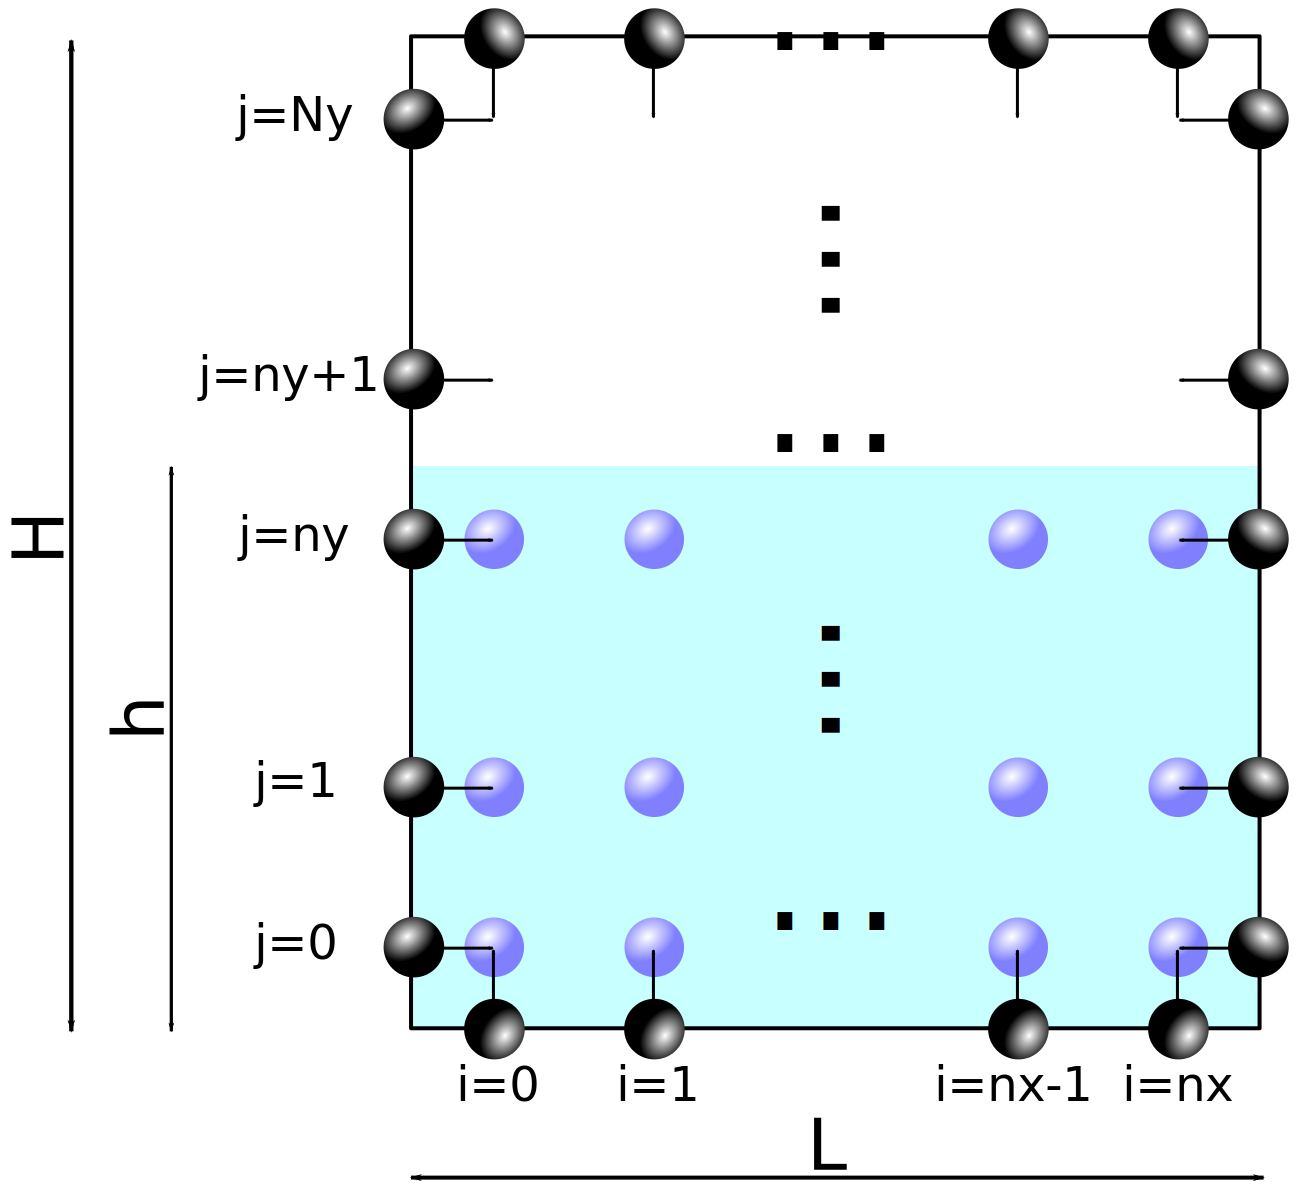
\includegraphics[width=0.8\textwidth]{lateral_water_1x_deleffe/particles}
  \caption{Particles packing scheme}
  \label{fig:examples:lateral_water_1x_deleffe:particles_packing}
\end{figure}
%
\subsection{Time discretization}
\label{ss:example:lateral_water_1x_deleffe:timing}
%
In \NAME the time is discretized in order to forward integrate it using the Leap-Frog scheme
documented in section \ref{ss:aquagpusph:leapfrog}. To perform the time discretization 2 main
magnitudes must be controlled, the simulation total time, and the time step. Also we can setup
a stabilization time.\rc
%
First for all create the XML definition file ``\textbf{Time.xml}'' with the section called
``Timing''. We want to run a simulation of 5 seconds without a stabilization stage and with a
time step such that is adapted in real time to fit to the criteria described in section
\ref{ss:sph:discrete:timestep}, that in this type of cases can be really useful due to in the
sloshing instant some particles can significantly accelerate getting high velocities, but
reducing the time step we can manage the situation. To set these options we add following tags
into the ``Timing'' section:
%
\begin{verbatim}
<Option name="SimulationStop" type="Time" value="5.0" />
<Option name="TimeStep" value="Variable"/>
<Option name="Stabilization" value="0.0"/>
\end{verbatim}
%
In order to improve the Courant number a division factor can be set as described in section
\ref{sss:XML:SPH}, in our case we will set a factor of 4 adding following option to the ``SPH''
section of the definition file ``SPH.xml'':
%
\begin{verbatim}
<Option name="DivDt" value="4.0" />
\end{verbatim}
%
\subsection{Output configuration}
\label{ss:example:lateral_water_1x_deleffe:output}
%
In order to post-process the simulation we want several output files:
%
\begin{enumerate}
	\item Sensor pressure: In the main output, and will require to set some sensors in the walls.
	\item Visualization: H5Part output files will be written in order to can perform
	visualizations with Paraview.
	\item Log file: In order to get a general view of the simulation process with relevant
	incidents, notifications and errors.
	\item Energy: An energy log along the simulation will be written too.
\end{enumerate}
%
In order to create the sensor 1 shown in the figure
\ref{fig:examples:lateral_water_1x_deleffe_scheme:scheme} we will add several measuring points in
order to can cover all the real sensor area\footnote{Must be noticed that in the case that kernel
height $h$ is greater than the sensor length, adding several points will not make effect since you
don't have resolution, but you can consider adding it in order to future resolution increasing.}.
To do it create the XML definition file ``Sensors.xml'' with the following content:
%
\begin{verbatim}
<?xml version="1.0" ?>
<sphInput>
	<Sensors>
		<FPS value="10000.0" />
		<Script file="/usr/share/aquagpusph/resources/OpenCL/Sensors" />
		<Sensor x="-0.45" y="0.09300" type="Interpolated" />
		<Sensor x="-0.45" y="0.09275" type="Interpolated" />
		<Sensor x="-0.45" y="0.09250" type="Interpolated" />
		<Sensor x="-0.45" y="0.09225" type="Interpolated" />
		<Sensor x="-0.45" y="0.09200" type="Interpolated" />
		<Sensor x="-0.45" y="0.09325" type="Interpolated" />
		<Sensor x="-0.45" y="0.09350" type="Interpolated" />
		<Sensor x="-0.45" y="0.09375" type="Interpolated" />
		<Sensor x="-0.45" y="0.09400" type="Interpolated" />
	</Sensors>
</sphInput>
\end{verbatim}
%
See the section \ref{sss:XML:Sensors} for further details about the options introduced. To set the
rest of output files edit the file ``\textbf{Time.xml}'' adding following options into section
``Timing'':
%
\begin{verbatim}
<Option name="Output" format="H5Part" type="FPS" value="30" />
<Option name="LogFiles" type="FPS" value="120" />
<Option name="EnFiles" type="FPS" value="120" />
<Option name="BoundsFiles" type="No" />
\end{verbatim}
%
Take care to don't set too high frequency of the visualization file output because huge hard disk
demand can be expected.
%
\subsection{Other options}
\label{ss:example:lateral_water_1x_deleffe:settings}
%
We may set some general \NAME settings, see section \ref{sss:XML:Settings} to learn more about the
general options. To set this options simply generate a file called ``Settings.xml'' with the following
content:
%
\begin{verbatim}
<?xml version="1.0" ?>
<sphInput>
	<Settings>
		<Verbose level="1" />
		<Start mode="0" />
	</Settings>
</sphInput>
\end{verbatim}
%
\subsection{Main XML definition file}
\label{ss:example:lateral_water_1x_deleffe:mainXML}
%
We have been generated following files:
%
\begin{itemize}
	\item Fluids.xml
	\item Movements.xml
	\item OpenCL.xml
	\item Sensors.xml
	\item Settings.xml
	\item SPH.xml
	\item Time.xml
	\item CreateMotions.py
	\item CreateParticles.py
	\item Particles.dat
	\item Move/6DOF.xml
	\item Move/6DOF.dat
	\item doc/lateral\_water\_1x.txt
\end{itemize}
%
The data files with the motions or the spatial discretization have been referenced into the corresponding
XML files, and the specific motion definition file ``Move/6DOF.xml'' has been referenced from the general
motions definition file ``Movements.xml'', but all the separately XML definition files must be grouped into
a general definition file that will load \NAME in order to setup the case. Create a file called
``\textbf{Main.xml}'' with the following content:
%
\begin{verbatim}
<?xml version="1.0" ?>
<sphInput>
	<Include file="Fluids.xml" />
	<Include file="Movements.xml" />
	<Include file="OpenCL.xml" />
	<Include file="Sensors.xml" />
	<Include file="Settings.xml" />
	<Include file="SPH.xml" />
	<Include file="Time.xml" />
</sphInput>
\end{verbatim}
%
This file don't contains any relevant data, only redirects \NAME to read all the other previously generated
files.
%
\subsection{Run the simulation}
\label{ss:example:lateral_water_1x_deleffe:running}
%
This case has been generated using relative paths\footnote{Relative paths provided into the configuration
files are ever relatives to the execution path, not to the XML path}, so must be executed in the root folder
where we have been generated it. Running the case is so quite easy, simply open a terminal in the folder where
you have the file ``\textbf{Main.xml}'' and execute
%
\begin{verbatim}
AQUAgpusph2D --input Main.xml --no-reassembly
\end{verbatim}
%
See section \ref{ss:running:launching} to learn more about the cases launch process and the messages that you
will receive while \NAME is running, and it's stored in the log file ``Log.html''. Depending on hardware used
the simulation can take from 2 hours to more than 10 hours, so consider reduce the resolution or the number of
neighbours in this case.
%
\subsection{Post-process the simulation}
\label{ss:example:lateral_water_1x_deleffe:postprocess}
%
\subsubsection{General}
\label{sss:example:lateral_water_1x_deleffe:postprocess:general}
%
Post-process can be divided in 2 main categories:
%
\begin{enumerate}
	\item Run time post-process
	\item Finished simulation post-process
\end{enumerate}
%
The first one has the advantage that can be performed while the simulation is running, and consist mainly on
plots of output data. The second one is mainly the visualization with the H5Part output.
%
\subsubsection{Run rime post-process}
\label{sss:example:lateral_water_1x_deleffe:postprocess:gnuplot}
%
In this case the main objective is to plot the pressure obtained on sensor 1 (see figure
\ref{fig:examples:lateral_water_1x_deleffe_scheme:scheme}), that is included in the data that can be processed
in run time. We will use intensively \textbf{gnuplot} and \textbf{awk} along this section.\rc
%
You can find more data about how is sensors file formatted in the section \ref{ss:aquagpusph:sensors}. Basically
we want to read the pressure data on each of the 9 measuring points placed around sensor 1 position, and plot
the average value along the time. With \textbf{awk}, get this pressure for each time instant written can be
performed typing in a terminal on the execution folder
%
\begin{verbatim}
awk '{p=$4+$9+$14+$19+$24+$29+$34+$39+$44;p=p/9.0; print $1,p}' Sensors.dat
\end{verbatim}
%
That loads the sensors output file ``Sensors.dat'', compute the required value for each time step, and return
2 columns with the time instants and the pressure obtained. Regarding the experimental data, pressure has been
measured in mbar, so we need to move it to Pa:
%
\begin{verbatim}
awk '{p=$2; print $1,100.0*p}' lateral_water_1x.txt
\end{verbatim}
%
So we can obtain, using \textbf{awk}, 2 files that contains the experimental and simulated pressures, so we only
need to create a \textbf{gnuplot} layout, that we can call ``\textbf{press.gnuplot}'' (place it in the root
folder), that uses internally \textbf{awk} to plot the desired data.
%
\begin{verbatim}
# Set plot options
set key
set grid
# Set x parameters
set xlabel "Time [s]"
set xtic
set xrange[0:5]
# Set left y parameters
set ylabel "Pressure [Pa]"
set ytic
set yrange[-1000:5000]
# Line styles
set style line 1 lt -1 lw 1
set style line 2 lt -1 lc rgb "red" lw 1

# Plot
plot \
"<awk '{p=$2; print $1,100.0*p}' doc/lateral_water_1x.txt" \
using 1:2 title 'Experimental' axes x1y1 with lines ls 2, \
"<awk '{p=$4+$9+$14+$19+$24+$29+$34+$39+$44;p=p/9.0; print $1,p}' Sensors.dat" \
using 1:2 title 'SPH' axes x1y1 with lines ls 1

pause 5
replot
reread
\end{verbatim}
%
The script shown above will plot the pressure data while it is available, reploting with in an interval of 5
seconds. In the figure \ref{fig:examples:lateral_water_1x_deleffe:sensors} you can see a pressure plot example
that you can expect using \textbf{gnuplot}.\rc
%
As you can see the results can be significantly improved as shown in the publication \citep{Maciaetal_PTP_2012}
where this simulation example was introduced, but is enough for our purposes. Feel free to play with the
parameters and see the effects.\rc
%
In the same way described you can plot the energy graphs.
%
\begin{figure}[h!]
  \centering
  \includegraphics[width=0.7\textwidth]{lateral_water_1x_deleffe/sensors_freeslip}
  \caption{Pressure register comparison between experimental and simulation data}
  \label{fig:examples:lateral_water_1x_deleffe:sensors}
\end{figure}
%
\subsubsection{Finished simulation post-process}
\label{sss:example:lateral_water_1x_deleffe:postprocess:paraview}
%
When the simulation has finished we can work over the H5Part output file. In this section we will use
\textbf{Paraview}. Remember that your \textbf{Paraview} needs the H5Part files loader plugin to can run.\rc
%
To start working executes Paraview, and go to ``File/Open''. A new window opens in order to select a file to
open, so select the output file ``Particles0.h5part'' and accept. At this point you still not seeing nothing
on the 3D view, but a new filter has been added to the pipeline, as you can see in the figure
\ref{fig:examples:lateral_water_1x_deleffe:paraviewfilter}. Below the pipeline you can find the options of
this filter, ensure that $Xarray$, $Yarray$ and $zArray$ are right, and press \textbf{Apply}. In the figure
\ref{fig:examples:lateral_water_1x_deleffe:paraviewfilteroptions} you can see how the options must be set.\rc
%
After that something is shown in the 3D view, our first objective will be separate in 3 different instances
the walls elements, the fluid particles, and the sensors, to do it we need to apply 4 filters, one to extract
solid that has $imove < 0$ flag, another one to extract fluid that has $imove > 0$ flag, and 2 more filters
for sensors that has $imove = 0$ flag.\rc
%
Go to \textbf{Filters/Common/Clip}, and a new filter depending on our original one is added. You can change
the filter name selecting it in the pipeline browser, and pressing ``F2'', set the name ``\textbf{Solid}''.
Now set the options in the object inspector as shown in figure
\ref{fig:examples:lateral_water_1x_deleffe:paraviewsolidfilter}, and press Apply. In 3D view only solid
elements are shown now.\rc
%
Before to get fluid particles we will format solid elements style. Change to the ``Display'' tab, and modify
``Color by'' option to \textbf{Solid Color}. Change the ``point size'' to \textbf{1.00} too in the ``Style''
section. You may see something similar to the presented on figure
\ref{fig:examples:lateral_water_1x_deleffe:paraviewsolid3D}.\rc
%
Selecting the H5Part file instnace apply now another \textbf{Clip} filter, but in this case select the
``Value'' \textbf{0.5}, and uncheck ``Inside Out'', naming to this new instance ``\textbf{Fluid}''.\rc
%
The fluid can be styled selecting ``Color by'' as \textbf{press}, and pressing ``Edit Color Map'' we can edit
the color mapping behaviour. In figure \ref{fig:examples:lateral_water_1x_deleffe:paraviewcolormap} the options
selected for the color map, in order to get the visualization shown in the figure
\ref{fig:examples:lateral_water_1x_deleffe:paraviewfluid3D} is shown. You can show the legend with the options
of the ``Color Legend'' tab of the same window.\rc
%
Finally add 2 new \textbf{Clip} filters, apply the first one to the H5Part loaded instance, with the ``Value''
\textbf{-0.5}, but with ``Inside Out'' unchecked, and apply the another filter to the first one with theç
``Value'' \textbf{0.5} and ``Inside Out'' checked. You can rename both filters as ``\textbf{Sensors}''.\rc
%
Sensors must be coloured with \textbf{press} too, but in this case the ``point size'' can be increased to and
hight value, for instance \textbf{3.0}.\rc
%
Finally you can change the background color with \textbf{Edit/View Settings...}. In this window you can also
set/unset the parallel projection\footnote{Is strongly recommended use parallel projection} and the
annotations.\rc
%
Now you have your visualization formatted, and you can start animating and saving images/videos.In the figure
\ref{fig:examples:lateral_water_1x_deleffe:paraviewanimation} you can see an example of an animation performed
with ParaView.\rc
%
You can additionally save a ParaView state that when you loads it apply automatically all the purposed filters.
%
\begin{figure}[ht!]
  \centering
  \includegraphics[width=0.3\textwidth]{lateral_water_1x_deleffe/paraviewfilter}
  \caption{Filter added to Paraview}
  \label{fig:examples:lateral_water_1x_deleffe:paraviewfilter}
\end{figure}
%
\begin{figure}[ht!]
  \centering
  \includegraphics[width=0.3\textwidth]{lateral_water_1x_deleffe/paraviewfilteroptions}
  \caption{H5Part loaded file options}
  \label{fig:examples:lateral_water_1x_deleffe:paraviewfilteroptions}
\end{figure}
%
\begin{figure}[ht!]
  \centering
  \includegraphics[width=0.3\textwidth]{lateral_water_1x_deleffe/paraviewsolidfilter}
  \caption{Solid Clip filter options}
  \label{fig:examples:lateral_water_1x_deleffe:paraviewsolidfilter}
\end{figure}
%
\begin{figure}[ht!]
  \centering
  \includegraphics[width=0.5\textwidth]{lateral_water_1x_deleffe/paraviewsolid3D}
  \caption{3D view with only the solid elements}
  \label{fig:examples:lateral_water_1x_deleffe:paraviewsolid3D}
\end{figure}
%
\begin{figure}[ht!]
  \centering
  \includegraphics[width=0.4\textwidth]{lateral_water_1x_deleffe/paraviewcolormap}
  \caption{Pressure color map options}
  \label{fig:examples:lateral_water_1x_deleffe:paraviewcolormap}
\end{figure}
%
\begin{figure}[ht!]
  \centering
  \includegraphics[width=0.5\textwidth]{lateral_water_1x_deleffe/paraviewfluid3D}
  \caption{3D view with the solid elements and the fluid particles}
  \label{fig:examples:lateral_water_1x_deleffe:paraviewfluid3D}
\end{figure}
%
\begin{figure}[ht!]
  \centering
  \includegraphics[width=0.7\textwidth]{lateral_water_1x_deleffe/animation_freeslip}
  \caption{Animation of the example for the first impact, frames 70-73, using free-slip boundary condition}
  \label{fig:examples:lateral_water_1x_deleffe:paraviewanimation}
\end{figure}
%
\subsection{Conclusions}
\label{ss:example:lateral_water_1x_deleffe:conclusions}
%
In this example is shown how to setup a case from scratch, that even though this is the the most complex way to
do it, is too easy to perform it. The example has been covered in detail, including the case setup, the
simulation launch, and the post-process.\rc
%
The unique tool that has been managed without text files has been Paraview, but if Paraview has been installed
with Python support, the work that we have been performed in the section
\ref{sss:example:lateral_water_1x_deleffe:postprocess:paraview} can be placed in a Python script, that is a text
file, so the entirely simulation could be easily scripted\footnote{\NAME package has internally scripted the
case with the CMake tool, that you can test it in comparing the built and installed versions, where all the paths
into the definition files and scripts are different}.\rc
%
In the results a typical Weakly compressible SPH (W-SPH) pressure noise can be noticed, but results have a good
quality.\rc
%
During the case generation we have set free-slip boundary condition along the walls because the Reynolds number
reached is so quite far from the real one (Dynamic viscosity has been artificially increased 400 times), but
we could considered that our Reynolds number is enough to set a no-slip boundary condition, with the hope that
we will receive a more stable simulation, and maybe with some better results. In the figure \ref{fig:examples:lateral_water_1x_deleffe:sensors_noslip} the pressure measured in the sensor 1 and the
simulation result using no-slip boundary condition is shown. You can compare the pressures computed using
free-slip, shown in the figure \ref{fig:examples:lateral_water_1x_deleffe:sensors}, and using no-slip,
shown in the figure \ref{fig:examples:lateral_water_1x_deleffe:sensors_noslip}, where can be noticed that the
best quality of the first one. In the figure \ref{fig:examples:lateral_water_1x_deleffe:paraviewanimation_noslip}
the same animation shown in the figure \ref{fig:examples:lateral_water_1x_deleffe:paraviewanimation} for the
free-slip is presented for the no-slip boundary condition.\rc
%
In this example we have generated all the needed files in order to perform the simulation, that are ready
installed on the system. Since we have been used relative directories to refer the files between them, we can
only execute our example from the generated location, but the installed version can be executed in whatever place
where we have permission to write. We will use this approach in the next example.\rc
%
The next example is heavy related with this one, but the boundary condition has been moved from boundary
integrals (formerly De Leffe or DeLeffe for the configuration files) to Ghost particles, that is probably the
most popular boundary condition generally used.
%
\begin{figure}[ht!]
  \centering
  \includegraphics[width=0.7\textwidth]{lateral_water_1x_deleffe/sensors_noslip}
  \caption{Pressure register comparison between experimental and simulation data, using no-slip boundary condition}
  \label{fig:examples:lateral_water_1x_deleffe:sensors_noslip}
\end{figure}
%
\begin{figure}[ht!]
  \centering
  \includegraphics[width=0.7\textwidth]{lateral_water_1x_deleffe/animation_noslip}
  \caption{Animation of the example for the first impact, frames 70-73, using no-slip boundary condition}
  \label{fig:examples:lateral_water_1x_deleffe:paraviewanimation_noslip}
\end{figure}
%